% GENERATED by make_paper_assets.py -- do not edit by hand.
\begin{figure}[t]
\centering
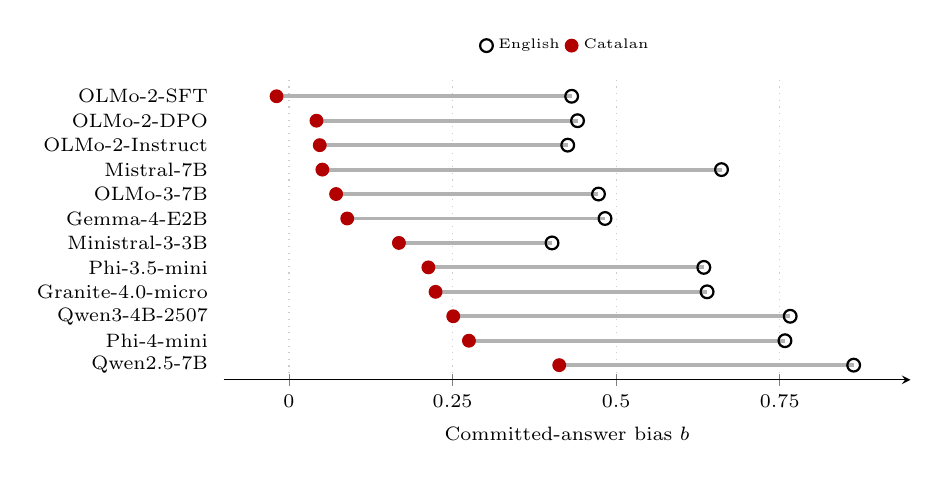
\begin{tikzpicture}
\begin{axis}[
  width=0.85\columnwidth, height=5.4cm, xmin=-0.1, xmax=0.95, ymin=0.4, ymax=12.7,
  xtick={0,0.25,0.5,0.75},
  ytick={12,11,10,9,8,7,6,5,4,3,2,1}, yticklabels={OLMo-2-SFT,OLMo-2-DPO,OLMo-2-Instruct,Mistral-7B,OLMo-3-7B,Gemma-4-E2B,Ministral-3-3B,Phi-3.5-mini,Granite-4.0-micro,Qwen3-4B-2507,Phi-4-mini,Qwen2.5-7B},
  xlabel={Committed-answer bias $b$},
  tick label style={font=\scriptsize}, label style={font=\scriptsize},
  axis lines=left, y axis line style={draw=none}, ytick style={draw=none},
  xmajorgrids, grid style={dotted, gray!40}, clip=false,
  legend style={at={(0.5,1.05)}, anchor=south, font=\tiny, draw=none, legend columns=2},
]
\draw[gray!60, line width=1.4pt] (axis cs:0.432,12) -- (axis cs:-0.019,12);
\draw[gray!60, line width=1.4pt] (axis cs:0.441,11) -- (axis cs:0.042,11);
\draw[gray!60, line width=1.4pt] (axis cs:0.426,10) -- (axis cs:0.047,10);
\draw[gray!60, line width=1.4pt] (axis cs:0.661,9) -- (axis cs:0.051,9);
\draw[gray!60, line width=1.4pt] (axis cs:0.473,8) -- (axis cs:0.072,8);
\draw[gray!60, line width=1.4pt] (axis cs:0.483,7) -- (axis cs:0.089,7);
\draw[gray!60, line width=1.4pt] (axis cs:0.402,6) -- (axis cs:0.168,6);
\draw[gray!60, line width=1.4pt] (axis cs:0.634,5) -- (axis cs:0.213,5);
\draw[gray!60, line width=1.4pt] (axis cs:0.639,4) -- (axis cs:0.224,4);
\draw[gray!60, line width=1.4pt] (axis cs:0.766,3) -- (axis cs:0.251,3);
\draw[gray!60, line width=1.4pt] (axis cs:0.758,2) -- (axis cs:0.275,2);
\draw[gray!60, line width=1.4pt] (axis cs:0.863,1) -- (axis cs:0.413,1);
\addplot[only marks, mark=o, mark size=2.3pt, black, thick] coordinates {(0.432,12) (0.441,11) (0.426,10) (0.661,9) (0.473,8) (0.483,7) (0.402,6) (0.634,5) (0.639,4) (0.766,3) (0.758,2) (0.863,1)};
\addlegendentry{English}
\addplot[only marks, mark=*, mark size=2.3pt, red!70!black] coordinates {(-0.019,12) (0.042,11) (0.047,10) (0.051,9) (0.072,8) (0.089,7) (0.168,6) (0.213,5) (0.224,4) (0.251,3) (0.275,2) (0.413,1)};
\addlegendentry{Catalan}
\end{axis}
\end{tikzpicture}
\caption{Committed-answer bias $b$ (Table~\ref{tab:catalan-mechanism}), English
versus Catalan, ordered by the Catalan value. It collapses toward zero for
OLMo-2 (all three variants) and Mistral-7B, but not for the remaining eight
checkpoints, which retain bias closer to their English value.}
\label{fig:catalan-mechanism}
\end{figure}
